\documentclass[a4paper, 10pt]{article}
\usepackage[utf8]{inputenc}
\usepackage{graphicx}
\usepackage{float}
\usepackage{geometry}
\usepackage[font=small, skip=0pt]{caption}
\usepackage{subcaption}
\usepackage{siunitx}
\usepackage{fancyhdr}
\geometry{margin=20mm}
\setlength{\textfloatsep}{4pt plus 1.0pt minus 2.0pt}
\setlength{\intextsep}{6.0pt plus 1.0pt minus 1.0pt}
\setlength{\belowcaptionskip}{-6pt}

\pagestyle{fancy}
\lhead{COMS30127 Rat Hippocampal Data}

\begin{document}

\section*{COMS30127 Lab M: Analysis of Hippocampal Data}

\subsection*{Introduction}
The hippocampus is a region of the brain that is responsible for spatial memory
and navigation. In order to investigate the function of neuronal cells within
the hippocampus, electrodes were attached to 4 neurons in the hippocampus of
rats, tasked with solving a simple maze.

\begin{figure}[H]
  \centering
  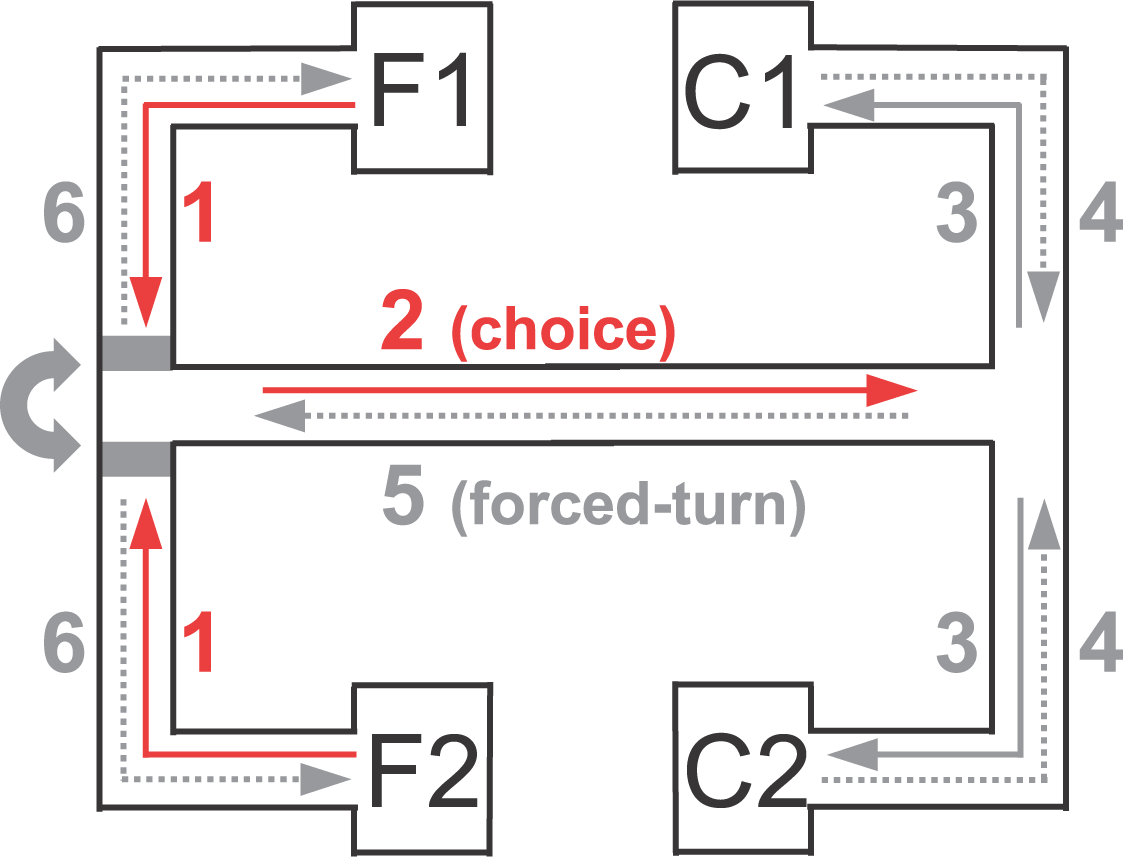
\includegraphics[width=0.5\textwidth]{rat_maze.png}
  \caption{A diagram detailing the task performed by the rats, from Jones MW, Wilson MA (2005). 'Theta Rhythms Coordinate Hippocampal–Prefrontal Interactions in a Spatial Memory Task'.}
  \label{fig:maze}
\end{figure}

\subsection*{Neuron Firing Positions}
\begin{figure}[H]
  \centering
  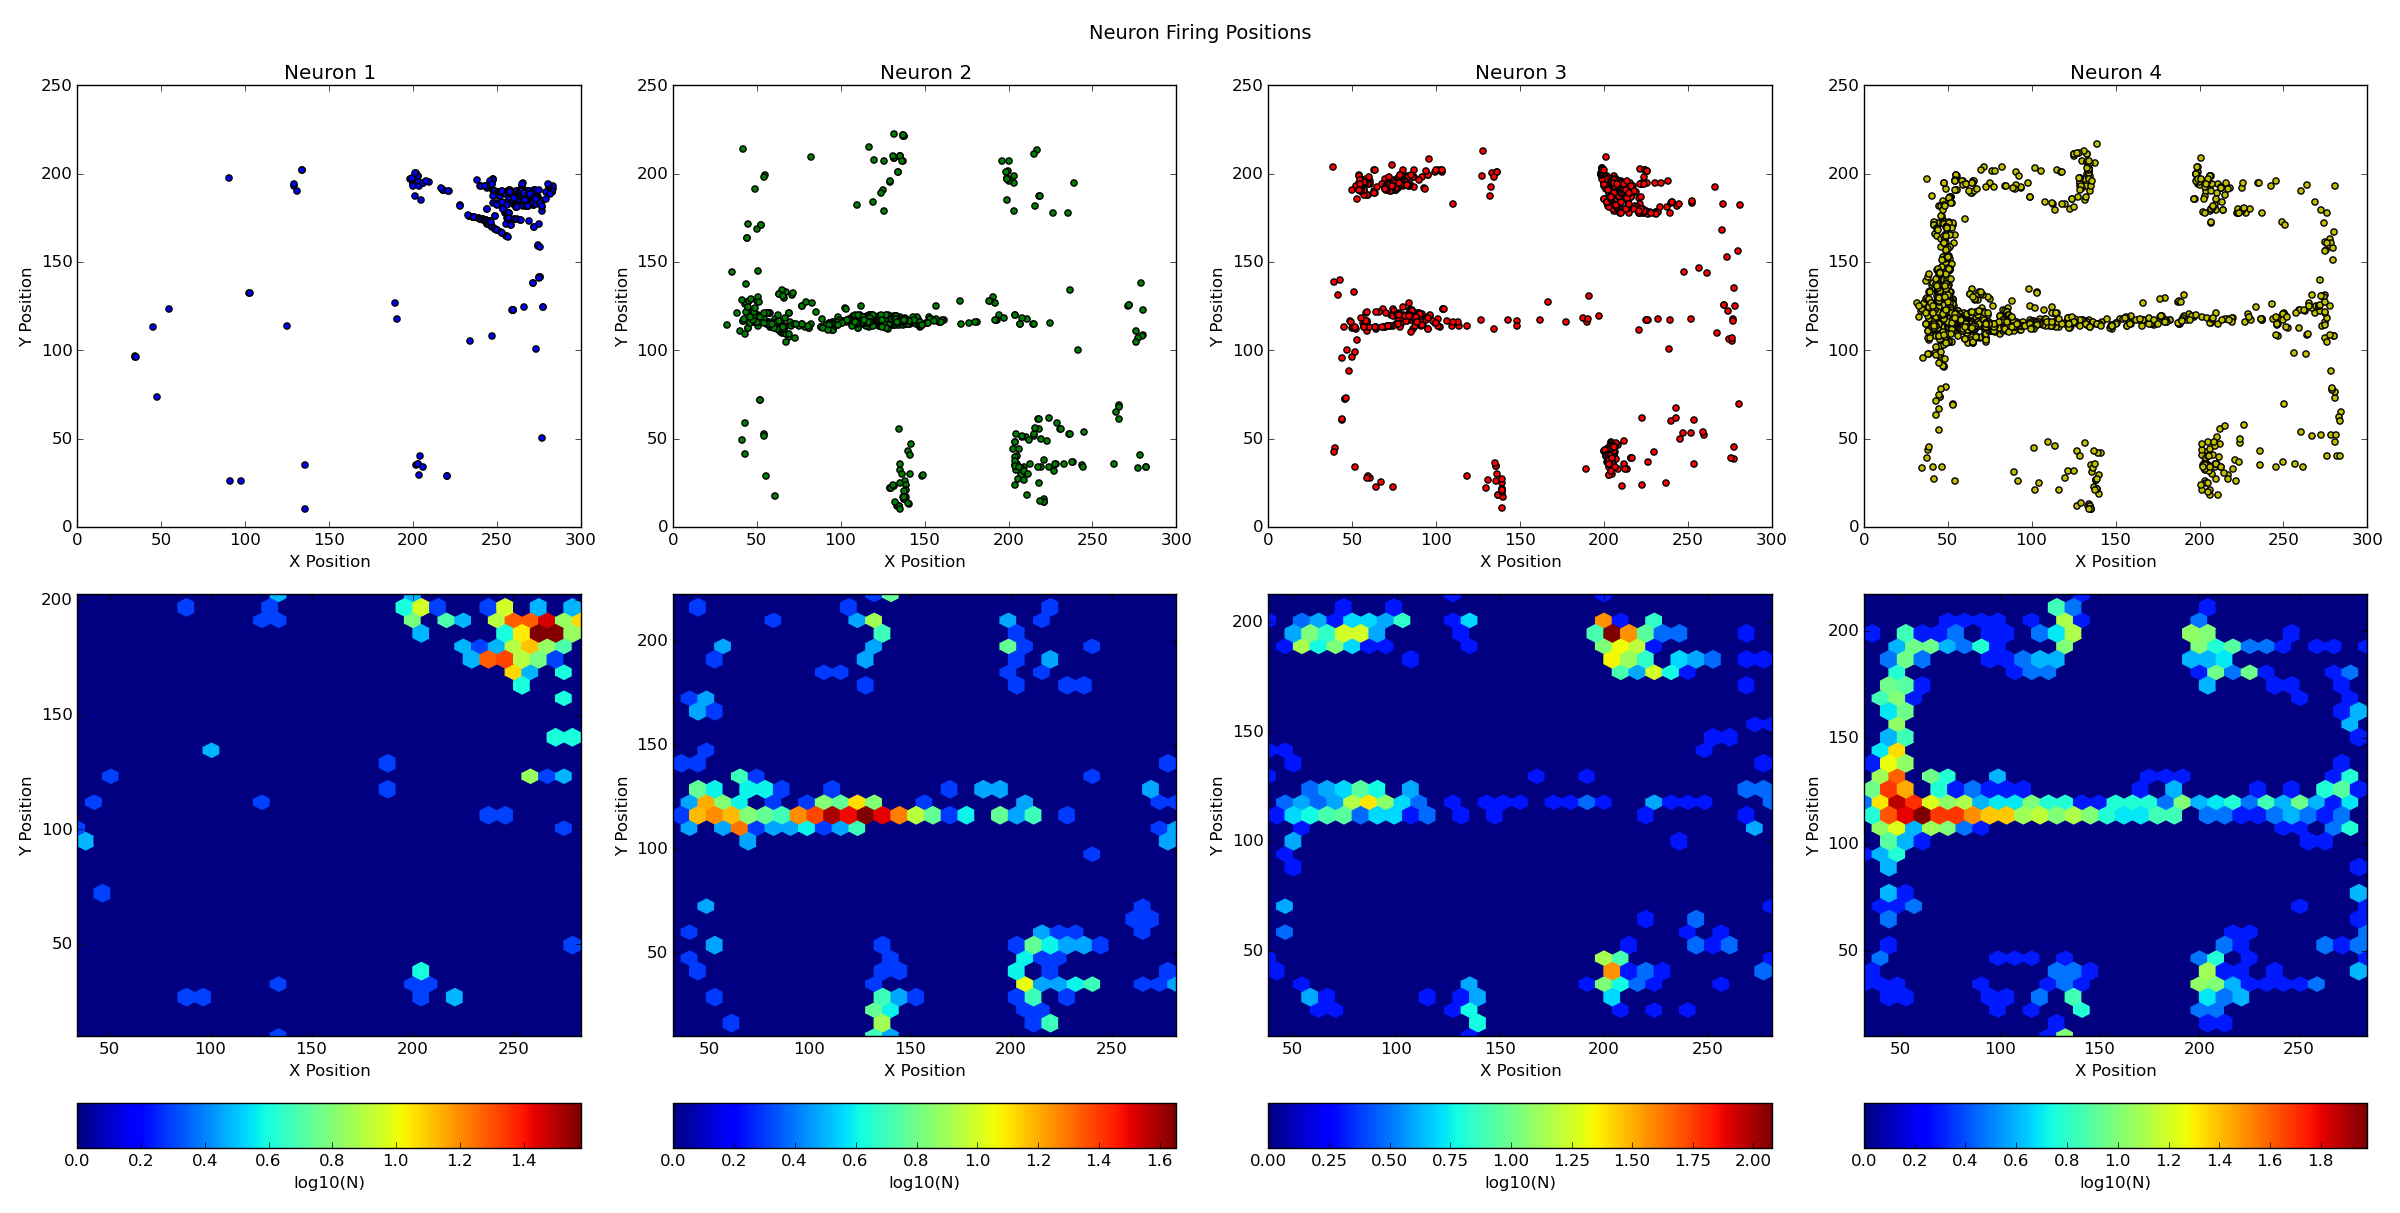
\includegraphics[width=1.0\textwidth]{neuron_pos_plot.png}
  \caption{Scatter plots and corressponding heatmaps showing the approximate location in which a spike occurred for each of the four recorded neurons.}
  \label{fig:posplot}
\end{figure}

Figure \ref{fig:posplot} shows the locations in which each neuron was most
active across multiple tests. The first neuron is active almost exclusively in
the upper right region of the maze, which suggests that this neuron is a place
cell. Place cells become active when an animal enters a corresponding place
field, but are otherwise relatively inactive. Place cells together are thought
to provide spatial processing. Neurons 2 and 4 appear to be closely
related. Neuron 2's activity is focused in the central arm of the maze. This
suggests it is involved with spatial or working memory; this neuron appears to
be involved in the recall process required to inform the choice made at the end
of the central arm. This conclusion is backed up by the activity of neuron 4,
that is most common at the end of the central arm and into the upper choice
arm. Neuron 4's apparent preference of the top arm suggests it is involved in
the decision process, using the information recalled by the second neuron. It
would be beneficial to find a corresponding neuron that showed a preference for
the opposite direction, to backup this hypothesis. Unfortunately, the function
of neuron 3 is not clear from these plots.

\subsection*{Neuron Auto-correlograms}
\begin{figure}[H]
  \centering
  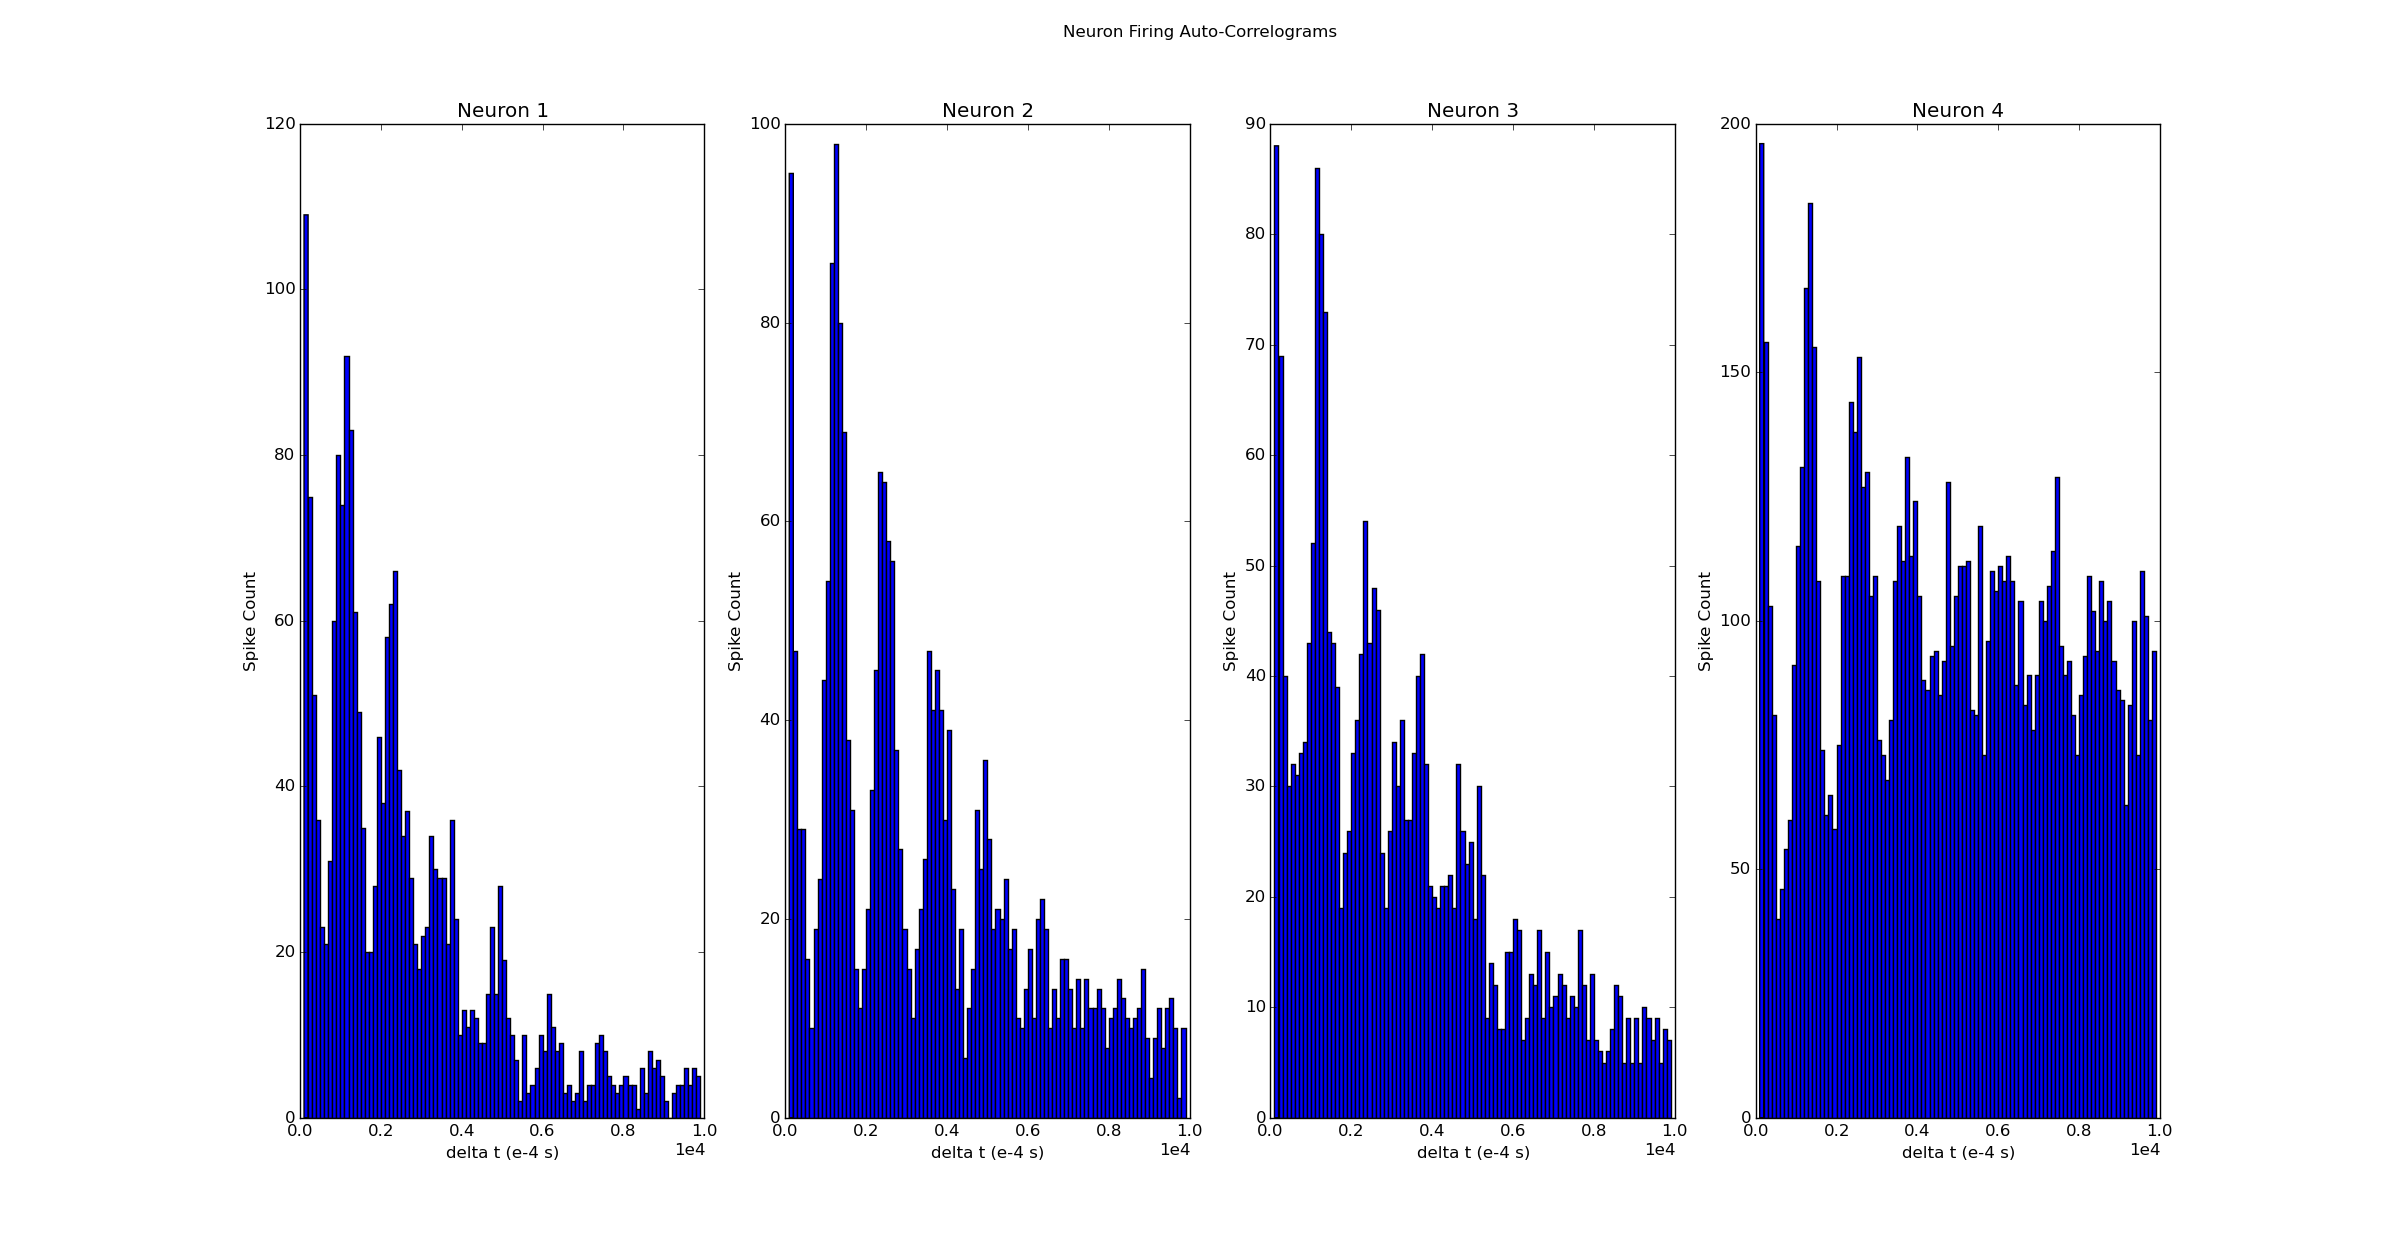
\includegraphics[width=1.0\textwidth]{neuron_acorr_plot.png}
  \caption{Auto-correlograms of neuron spike trains.}
  \label{fig:acorr}
\end{figure}

Figure \ref{fig:acorr} reveals an underlying frequency of approximately
\SI{10}{\hertz}. This shows itself as peaks representing the top half of a sine
wave with a period of roughly \SI{0.1}{\second}. This shows the presence of the
theta rhythm in the hippocampus, which is thought to be related to the
context-dependant retrieval of episodes from memory\footnote{Hasselmo, ME;
  Eichenbaum H (2005). 'Hippocampal mechanisms for the context-dependent
  retrieval of episodes'}, or as a mechanism for the relative timing of
disparate neural networks\footnote{Jones MW, Wilson MA (2005). 'Theta Rhythms
  Coordinate Hippocampal–Prefrontal Interactions in a Spatial Memory
  Task'}. Interestingly, neuron 4 exhibits a superimposed lower frequency signal
of approximately \SI{1}{\hertz}, a small portion of which is visible in the
plot.

\subsection*{Neuron Cross-correlograms}
\begin{figure}[H]
  \centering
  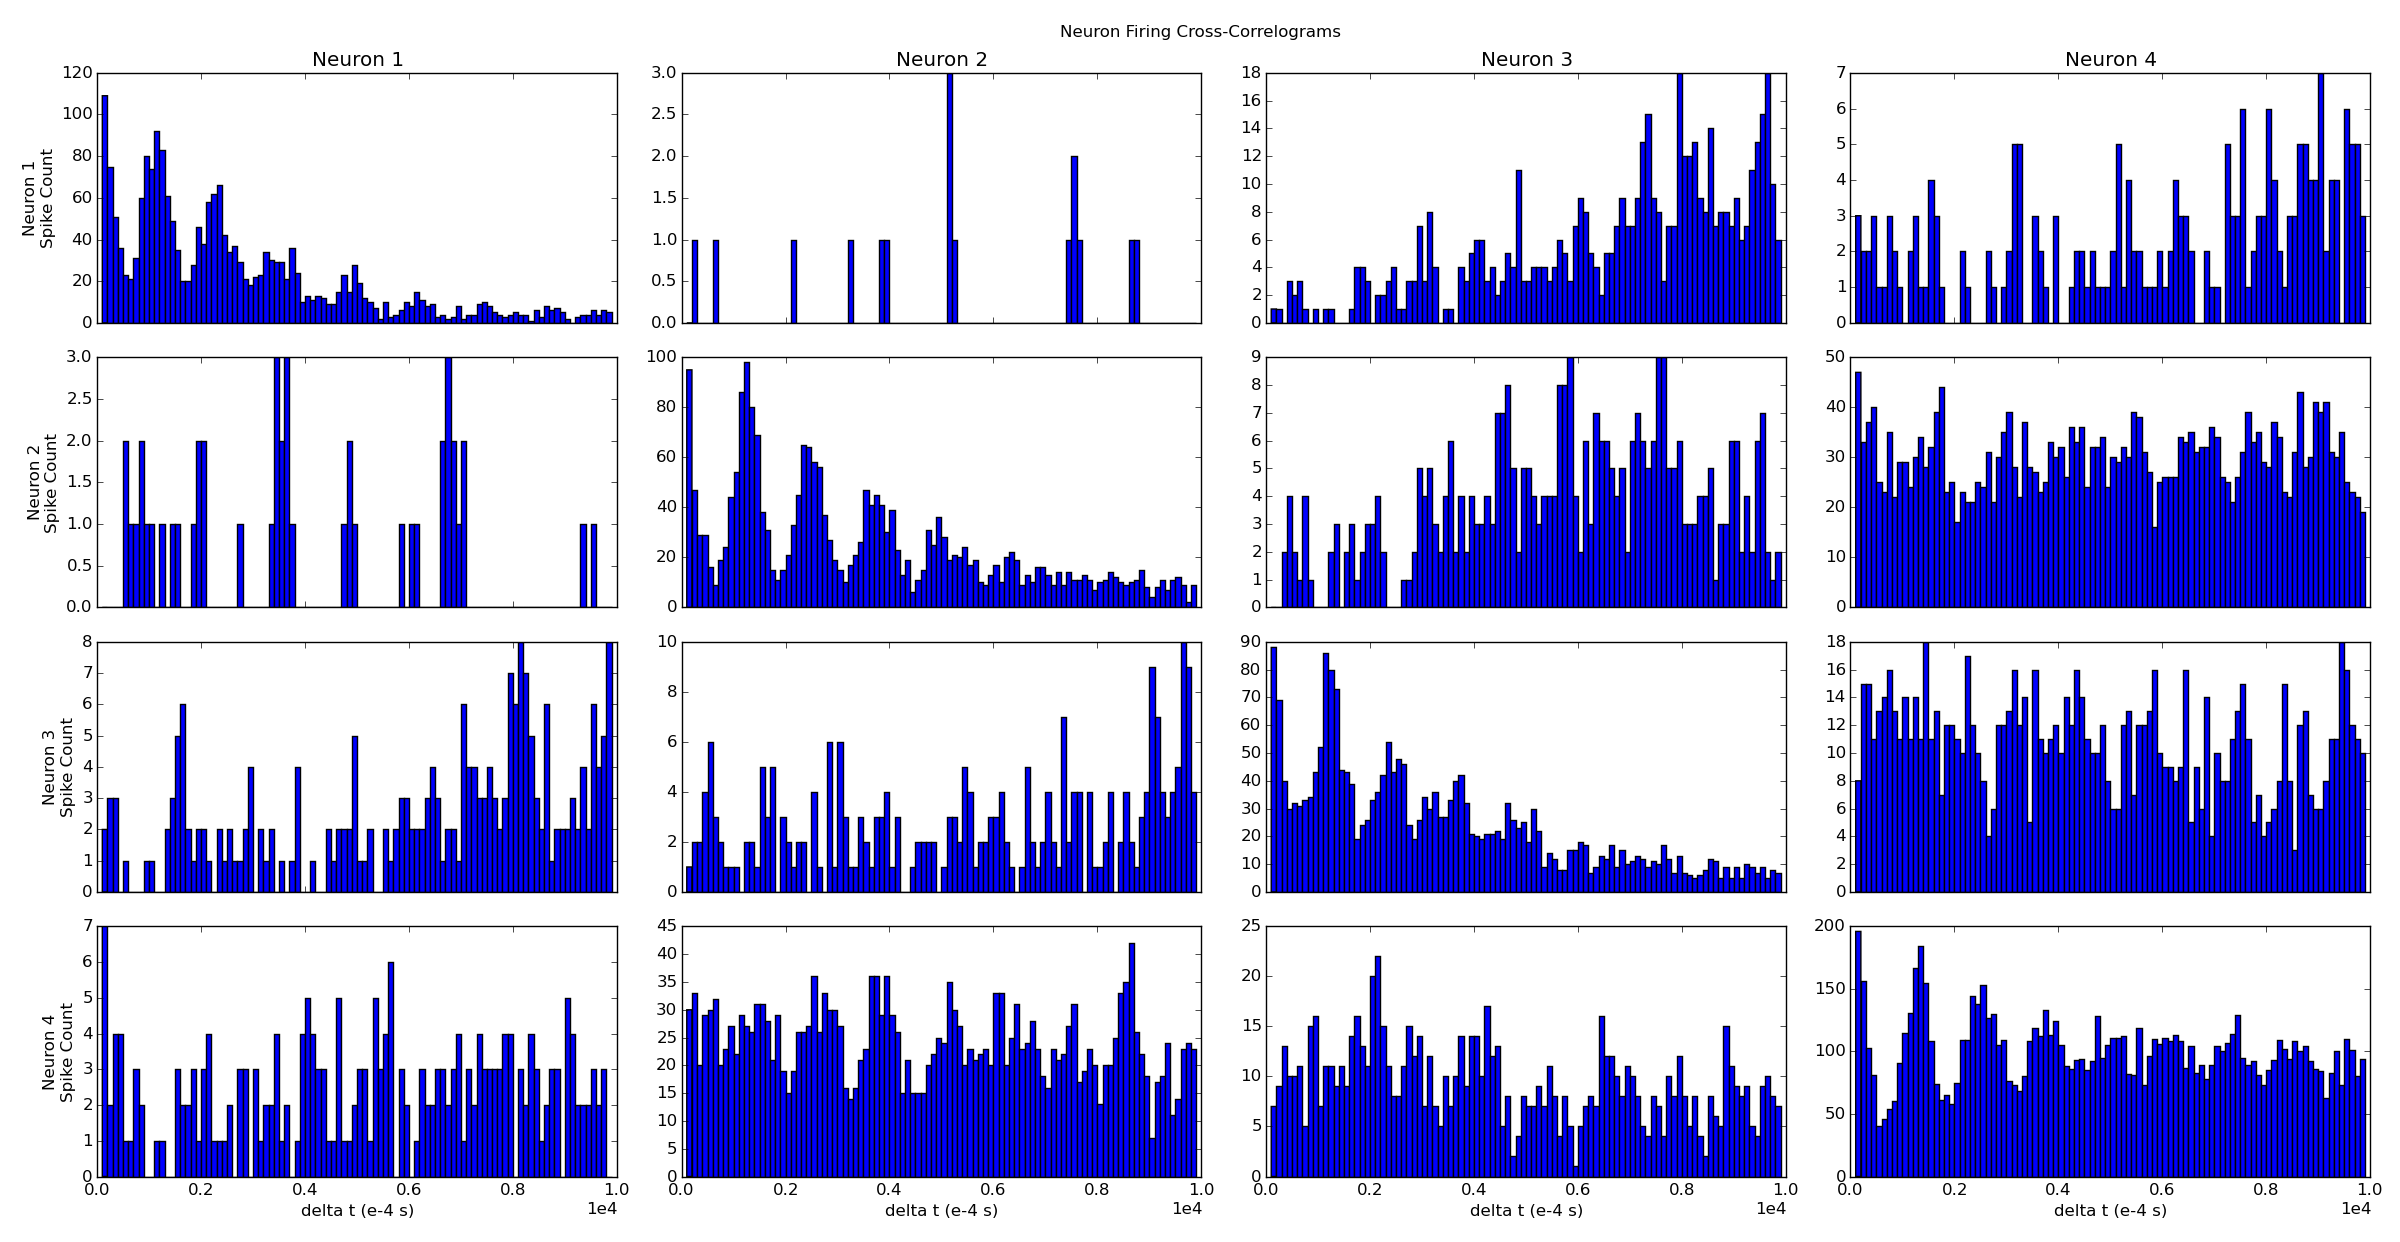
\includegraphics[width=1.0\textwidth]{neuron_xcorr_plot.png}
  \caption{Cross-correlograms of selected neuron spike train pairs.}
  \label{fig:xcorr}
\end{figure}

Figure \ref{fig:xcorr} shows some cross-correlograms of neuron
pairs. Unfortunately, the theta rhythms present in all the recorded neurons
obscure any meaningful relationships that may otherwise have been revealed
here. A quick evaluation of the two plots above shows that Neurons 2 and 4 have
little correlation, with a fairly even set of histogram heights. Neurons 1 and 3
on the other hand shows some correlation around the \SI{0.8}{\second} mark.

\subsection*{Conclusion}

In conclusion, from my analysis of the hippocampal data I have determined that
neuron 1 is a place cell, with a place field corresponding to the start position
F2. Neuron 2 appears to be related to recall from working memory, where it
informs the choice made by neuron 4, which fires most often when making the
right turn at the end of the central arm. I expect there to be corresponding
neuron(s) not recorded in the data that have a preference to the opposite
turn. The recall of neuron 2 would cause either neuron 4 or the related neurons
to fire more rapidly, influencing the choice of the rat. Auto-correlograms of
the recorded spike trains show the presence of theta-rhythms in the hippocampus,
which are thought to enable retrieval of episodes from memory based on context,
which would backup these ideas. The presence of a low frequency signal in neuron
4 is interesting, although it's purpose is unclear. Unfortunately, due to the
presence of these theta-rhythms, the cross-correlograms of neuron pairs are
somewhat inconclusive, and cannot be used to backup the argument of the relation
of neurons 2 and 4.

\end{document}
